\chapter{Intervalový odhad}

\section{Interval spolehlivosti}

\subsection{Definice intervalu spolehlivosti}

\begin{definition}[Interval spolehlivosti]
Uvažujme náhodný výběr $X_1, ..., X_n$ z populace $f(\cdot, \theta)$. Nechť $T_1 = \mathfrak{t}_1(X_1, ..., X_n)$ a $T_2 = \mathfrak{t}_2(X_1, ..., X_n)$ představují dvě statistiky, které splňují podmínku $T_1 \le T_2$ a pro které platí $P_{\theta}[T_1 < \tau(\theta) < T_2] \equiv \gamma$, kde $\gamma$ není funkcí $\theta$. Náhodný interval $(T_1, T_2)$ nazýváme 100$\gamma$ procentním intervalem spolehlivosti pro $\tau(\theta)$ a $T_1$ resp. $T_2$ nazýváme jeho dolním resp. horním limitem. Hodnotu  $(t_1, t_2)$ náhodného intervalu $(T_1, T_2)$ taktéž nazýváme 100$\gamma$ procentním intervalem spolehlivosti pro $\tau(\theta)$.
\end{definition}

Jedna ze statistik $\mathfrak{t}_1(X_1, ..., X_n)$ a $\mathfrak{t}_2(X_1, ..., X_n)$ může být konstantou.

\begin{definition}[Jednostranný interval spolehlivosti]
Uvažujme náhodný výběr $X_1, ..., X_n$ z populace $f(\cdot, \theta)$. Nechť $T_1 = \mathfrak{t}_1(X_1, ..., X_n)$ je statistika, pro kterou platí $P_{\theta}[T_1 < \tau(\theta)] \equiv \gamma$. Pak $T_1$ nazýváme levostranným limitem spolehlivosti pro $\tau(\theta)$. Podobně, je-li $T_2 = \mathfrak{t}_2(X_1, ..., X_n)$ statistika, pro kterou platí $P_{\theta}[\tau(\theta) < T_2]$, pak nazýváme $T_2$ pravostranným intervalem spolehlivosti pro $\tau(\theta)$.
\end{definition}

\begin{example}
Uvažujme náhodný výběr z populace $f(x, \theta) = \phi_{0, 9}(x)$. Definujme $T_1 = \mathfrak{t}_1(X_1, ..., X_n) = \overline{X} - \frac{6}{\sqrt{n}}$ a $T_2 = \mathfrak{t}_2(X_1, ..., X_n) = \overline{X} + \frac{6}{\sqrt{n}}$. Pak $(T_1, T_2)$ představuje interval spolehlivosti pro $\tau(\theta) = \theta$ s koeficientem spolehlivosti $\gamma = P_{\theta}[\overline{X} - \frac{6}{\sqrt{n}} < \theta < \overline{X} + \frac{6}{\sqrt{n}}] = P_{\theta}[-2 < \frac{\overline{X} - \theta}{3 / \sqrt{n}} < 2] = \Phi(2) - \Phi(-2) = 0.9772 - 0.0228 = 0.9544$. Jestliže by střední hodnota náhodného výběru o, řekněme, 25 prvcích byla 17.5, pak je interval $(17.5 - \frac{6}{\sqrt{25}}, 17.5 + \frac{6}{\sqrt{25}})$ nazýván 95.44 procentním intervalem spolehlivosti pro $\theta$.
\end{example}

Z daného 100$\gamma$ procentního intervalu spolehlivosti pro $\theta$ je možné odvodit 100$\gamma$ procentní interval spolehlivosti pro $\tau(\theta)$ za předpokladu, že $\tau(\cdot)$ je striktně monotonní funkcí. Jestliže je $\tau(\cdot)$ rostoucí funkcí a $(T_1, T_2)$ je 100$\gamma$ procentním intervalem spolehlivosti pro $\theta$, pak $(\tau(T_1), \tau(T_2))$ je 100$\gamma$ procentním intervalem spolehlivosti pro $\tau(\theta)$, protože
\begin{equation*}
P_{\theta}[\tau(T_1) < \tau(\theta) < \tau(T_2)] = P_{\theta}[T_1 < \theta < T_2]
\end{equation*}

Stejně jako v případě bodového odhadu čelíme dvojímu problému. Prvním problémem je definování metod pro nalezení intervalu spolehlivosti. Druhým problémem je nalezení vhodného kritéria pro porovnání všech možných intervalů spolehlivosti. Tímto se dostáváme k následující kapitole.

\subsection{Centrální veličina}

\begin{definition}[Centrální veličina]
Uvažujme náhodný výběr $X_1, ..., X_n$ z populace $f(x, \theta)$. Definujme $Q = \mathit{q}(X_1, ..., X_n; \theta)$. Jestliže pravděpodobnostní funkce náhodné veličiny $Q$ nezávisí na $\theta$, pak ji nazýváme centrální veličinou.
\end{definition}

\begin{example}
Uvažujme náhodný výběr $X_1, ..., X_n$ z populace $f(x, \theta) = \phi_{\theta, 9}(x)$. $\overline{X} - \theta$ je centrální veličinou, protože $\overline{X} - \theta$ sleduje normální rozdělení se střední hodnotou nula a rozptylem $9/n$. Také $\frac{\overline{X} - \theta}{3/ \sqrt{n}}$ je centrální veličinou, protože sleduje normalizované normální rozdělení. Naproti tomu $\overline{X}/ \theta$ není centrální veličinou, protože sleduje normální rozdělení s jednotkovou střední hodnotou a rozptylem $9/\theta^2n$.
\end{example}

\begin{definition}[Metoda centrální veličiny]
Jestliže $Q = \mathit{q}(X_1, ..., X_n; \theta)$ je centrální veličinou, pak pro libovolné $0 < \gamma < 1$ existují $q_1$ a $q_2$ taková, že $P[q_1 < Q < q_2] = \gamma$. Jestliže pro libovolné realizace náhodného výběru $x_1, ..., x_n$ platí $q_1 < \mathit{q}(x_1, ..., x_n; \theta) < q_2$ tehdy a jen tehdy, jestliže $\mathfrak{t}_1(x_1, ..., x_n) < \tau(\theta) < \mathfrak{t}_2(x_1, ..., x_n)$\footnote{Připomeňme, že funkce $\mathit(t)_1$ a $\mathit(t)_2$ nezávisí na $\theta$.}, pak $(T_1, T_2)$ představuje 100$\gamma$ procentní interval spolehlivosti pro $\tau(\theta)$, kde $T_i = \mathfrak{t}_i(X_1, ..., X_n)$ pro $i = 1, 2$.
\end{definition}

Je zřejmé, že $q_1$ a $q_2$ jsou nezávislé na $\theta$, protože $Q$ je taktéž nezávislé na $\theta$.

Pro každou hodnotu $\gamma$ existuje mnoho možných párů $q_1$ a $q_2$, které splňují podmínku $P[q_1 < Q < q_2] = \gamma$. Různá $q_1$ a $q_2$ definují různé funkce $\mathfrak{t}_1$ a $\mathfrak{t}_2$. Je zřejmé, že preferujeme taková $\mathfrak{t}_1$ a $\mathfrak{t}_2$, která jsou si pokud možno co ``nejblíže''. Definujme tuto ``blízkost'' jako $\mathfrak{t}_2(X_1, ..., X_n) - \mathfrak{t}_1(X_1, ..., X_n)$. Jestliže vzdálenost mezi $\mathfrak{t}_1$ a $\mathfrak{t}_2$ nemá charakter náhodné veličiny, pak vybereme taková $q_1$ a $q_2$, která tuto vzdálenost minimalizují. Pokud má tato vzdálenost charakter náhodné veličiny, pak vybereme taková $q_1$ a $q_2$, která minimalizují její střední hodnotu.

Základním požadavkem na centrální veličinu je, že nerovnost $\{q_1 < \mathit{q}(x_1, ..., x_n; \theta) < q_2\}$ lze přepsat do tvaru $\{\mathfrak{t}_1(x_1, ..., x_n) < \tau(\theta) < \mathfrak{t}_2(x_1, ..., x_n)\}$ pro libovolnou realizaci náhodného výběru $x_1, ..., x_n$. Tato vlastnost však není implikována výše uvedenou definici centrální veličiny.

\begin{example}
Uvažujme náhodný výběr $X_1, ..., X_n$ z $\phi_{\theta, 1}$. Nechť $\tau(\theta) = \theta$. Náhodná veličina $Q = \mathit{q}(X_1, ..., X_n; \theta) = \frac{\overline{X} - \theta}{\sqrt{1}{n}}$ sleduje normalizované normální rozdělení, a proto představuje centrální veličinu. Platí $f_Q(q) = \phi(q)$. Pro dané $0 < \gamma < 1$ existuje nekonečně párů $q_1$ a $q_2$, které splňují podmínku $P[q_1 < Q < q_2] = \gamma$.

$\{q_1 < \frac{\overline{x} - \theta}{\sqrt{1/n}} < q_2\}$ implikuje $\{\overline{x} - q_2\sqrt{1/n} < \theta < \overline{x} - q_1 \sqrt{1/n}\}$. Proto je interval  $\{\overline{X} - q_2\sqrt{1/n} < \theta < \overline{X} - q_1 \sqrt{1/n}\}$ 100$\gamma$ procentním intervalem spolehlivosti pro $\theta$. Délka tohoto intervalu je $(\overline{X} - q_1\sqrt{1/n}) - (\overline{X} - q_2 \sqrt{1/n}) = (q_2 - q_1)\sqrt{1/n}$ a je proto nejkratší pro nejmenší hodnotu $q_2 - q_1$ při splnění podmínky $\gamma = P[q_1 < Q < q_2] = \Phi(q_2) - \Phi(q_1)$. Délka tohoto intervalu tak dosahuje minima pro $q_1 = - q_2$.
\end{example}

\section{Náhodný výběr z normálního rozdělení}

\subsection{Interval spolehlivosti pro střední hodnotu}

Uvažujme náhodný výběr $X_1, ..., X_n$ z populace, která sleduje normální rozdělení, jejíž střední hodnotu ani rozptyl neznáme. To znamená, že $\theta = (\mu, \sigma)$ a $\tau(\theta) = \mu$. Náhodná veličina $\frac{\overline{X} - \mu}{\sigma / \sqrt{n}}$ sleduje normované normální rozdělení, a proto je centrální veličinou. Nicméně $\{q_1 < \frac{\overline{x} - \mu}{\sigma / \sqrt{n}} < q_2 \}$ nelze převést do tvaru $\{\mathfrak{t}_1(x_1, ..., x_n) < \mu < \mathfrak{t}_1(x_1, ..., x_n)\}$. Důvodem je, že $\frac{\overline{X} - \mu}{\sigma / \sqrt{n}}$ obsahuje neznámé $\sigma$. Připomeňme, že hledáme centrální veličinu, jejíž jedinou neznámou je $\mu$. Nicméně víme, že
\begin{equation*}
\frac{\frac{\overline{X} - \mu}{\frac{\sigma}{\sqrt{n}}}}{\sqrt\frac{\sum_{i = 1}^n (X_i - \overline{X})^2}{(n - 1)\sigma^2}} = \frac{\overline{X} - \mu}{S_n / \sqrt{n}}
\end{equation*}
sleduje studentovo rozdělení s $n - 1$ stupni volnosti\footnote{Připomeňme, že $S_n^2 = \frac{\sum_{i = 1}^2}{n - 1}$.}. Pravděpodobnostní funkce náhodné veličiny $\frac{\overline{X} - \mu}{S_n / \sqrt{n}}$ je tak nezávislá na $\mu$ a $\sigma^2$, a proto se jedná o centrální veličinu. Nerovnosti $\{q_1 < \frac{\overline{x} - \mu}{\mathit{s} / \sqrt{n}} < q_2\}$ implikují $\{\overline{x} - q_2\frac{\mathit{s}}{\sqrt{n}} < \mu < \overline{x} - q_1\frac{\mathit{s}}{\sqrt{n}}\}$, kde $q_1$ a $q_2$ splňují podmínku $P[q_1 < \frac{\overline{X} - \mu}{S_n / \sqrt{n}} < q_2] = \gamma$. Proto je $(\overline{X} - q_2 \frac{S_n}{\sqrt{n}}, (\overline{X} - q_1 \frac{S_n}{\sqrt{n}})$ 100$\gamma$ procentním intervalem spolehlivosti pro $\mu$. Délka tohoto intervalu je $\frac{q_2 - q_1}{S / \sqrt{n}}$, což je náhodná veličina. Pro libovolný náhodný výběr je jeho délka minimalizována pro nejmenší $q_2 - q_1$. To je splněno pro $q_1 = - q_2$, jak dokazuje následující text.

Naším cílem je minimalizovat
\begin{equation*}
L = \frac{S_n}{\sqrt{n}}(q_2 - q_1)
\end{equation*} 
při splnění podmínky
\begin{equation*}
\int_{q_1}^{q_2} f_T(t) dt = \gamma
\end{equation*}
kde $f_T(t)$ je pravděpodobnostní funkce studentova rozdělení s $n - 1$ stupni volnosti. Derivací výše uvedené rovnice podle $q_1$ získáme
\begin{equation*}
f_T(q_2)\frac{d q_2}{d q_1} - f_T(q_1) = 0
\end{equation*}
Abychom minimalizovali $L$, musíme řešit rovnici $\frac{dL}{d q_1}$, tj.
\begin{equation*}
\frac{dL}{dq_1} = \frac{S_n}{\sqrt{n}}\left(\frac{d q_2}{d q_1} - 1 \right) = 0
\end{equation*}
Zároveň však platí
\begin{equation*}
\frac{S_n}{\sqrt{n}}\left(\frac{d q_2}{d q_1} - 1\right) = \frac{S_n}{\sqrt{n}}\left(\frac{f_t(q_1)}{f_t(q_2)} - 1\right) = 0
\end{equation*}
Tato rovnost je tedy splněna pro $f_T(q_2) = f_T(q_1)$, což v kontextu symetrického studentova rozdělení znamená $q_1 = - q_2$.

\subsection{Interval spolehlivosti pro rozptyl}

Uvažujme náhodný výběr $X_1, ..., X_n$ z populace, která sleduje normální rozdělení, jejíž střední hodnotu ani rozptyl neznáme. Víme, že náhodná veličina
\begin{equation*}
Q = \frac{\sum_{i = 1}^n (X_i - \overline{X})^2}{\sigma^2} = \frac{(n - 1)S_n^2}{\sigma^2}
\end{equation*}
sleduje chi-kvadrát rozdělení s $n - 1$ stupni volnosti. Náhodná veličina $Q$ je tedy centrální veličinou. Je zřejmé, že $\big\{q_1 < \frac{(n - 1)\mathit{s}^2}{\sigma^2} < q_2 \big\}$ implikuje $\big\{\frac{(n - 1) \mathit{s}^2}{q_2} < \sigma^2 < \frac{(n - 1)s^2}{q_1}\big\}$. To znamená, že $\left(\frac{(n - 1)S_n^2}{q_2}, \frac{(n - 1)S_n^2}{q_1} \right)$ je 100$\gamma$ procentní interval spolehlivosti pro $\sigma^2$, $q_1$ a $q_2$ splňují podmínku $P[q_1 < Q < q_2] = \gamma$.

$q_1$ a $q_2$ jsou často zvoleny tak, aby $P[Q < q_1] = P[Q > q_2] = \frac{1 - \gamma}{2}$. O takovémto intervalu spolehlivosti pak hovoříme jako o intervalu spolehlivosti se shodnými chvosty.

Další možností je nalézt taková $q_1$ a $q_2$, která minimalizují délku intervalu $L$, kde
\begin{equation*}
L = (n - 1)S_n^2 \left(\frac{1}{q_1} - \frac{1}{q_2}\right)
\end{equation*}
Nechť $f_Q(q)$ představuje pravděpodobnostní funkci chi-kvadrát rozdělení s $n - 1$ stupni volnosti. Derivací podmínky
\begin{equation*}
\int_{q_1}^{q_2} f_Q(q)dq = \gamma
\end{equation*}
dle $q_1$ získáváme
\begin{equation*}
\frac{dq_2}{dq_1}f_Q(q_2) - f_Q(q_1) = 0
\end{equation*}
a proto
\begin{equation*}
\frac{dL}{dq_1} = (n - 1)S_n^2\left(-\frac{1}{q_1^2} + \frac{1}{q_2^2}\frac{dq_2}{dq_1}\right) = (n - 1)S_n^2\left(- \frac{1}{q_1^2} + \frac{1}{q_2^2}\frac{f_Q(q_1)}{f_Q(q_2)}\right) = 0
\end{equation*}
což implikuje $q_1^2 f_Q(q_1) = q_2^2 f_Q(q_2)$. Délka intervalu spolehlivosti tak bude minimální pro $q_1$ a $q_2$ taková, že
\begin{equation*}
q_1^2 f_Q(q_1) = q_2^2 f_Q(q_2)
\end{equation*}
při splnění podmínky
\begin{equation*}
\int_{q_1}^{q_2} f_Q(q) dq = \gamma
\end{equation*}
Řešení pro $q_1$ a $q_2$ lze nalézt pomocí numerické integrace.

Závěrem uveďme, že pro libovolná $q_1$ a $q_2$ taková, že $\int_{q_1}^{q_2}f_Q(q)dq = \gamma$ představuje $\left(\sqrt{\frac{(n - 1)S_n^2}{q_2}}, \sqrt{\frac{(n - 1)S_n^2}{q_1}}
\right)$ 100$\gamma$ procentní interval spolehlivosti pro $\sigma$.

\subsection{Region spolehlivosti pro střední hodnotu a rozptyl}

Při konstrukci regionu spolehlivosti pro střední hodnotu $\mu$ a rozptyl $\sigma^2$ normálního rozdělení by se na první pohled mohlo zdát, že stačí rutinně aplikovat postup předešlých dvou kapitol. To znamená, že např. pro konstrukci 95 procentního regionu spolehlivosti ilustrovaného obrázkem (\ref{conf-interval-mu-sigma_a}) by stačilo použít vztahů
\begin{gather*}
P\left[\overline{X} - t_{0.975}\frac{S_n^2}{n} < \mu < \overline{X} + t_{0.975}\frac{S_n^2}{n}\right] = 0.95\\
P\left[\frac{(n - 1)S_n^2}{\chi_{0.975}^2} < \sigma^2 < \frac{(n - 1)S_n^2}{\chi_{0.025}^2}\right] = 0.95
\end{gather*}
kde $t_{0.975}$ představuje 97.5 procentní kvantil studentova rozdělení s $n - 1$ stupni volnosti a $\chi_{0.025}^2$ resp. $\chi_{0.975}^2$ představuje 2.5 resp. 97.5
 procentní kvantil chi-kvadrát rozdělení s $n - 1$ stupni volnosti. Region ilustrovaný obrázkem (\ref{conf-interval-mu-sigma_a}) je sice regionem spolehlivosti pro $(\mu, \sigma^2)$, ale jeho koeficient spolehlivosti neznáme. Víme pouze, že tento koeficient není $0.95^2$, protože výše uvedené dva vztahy nejsou nezávislé.

\begin{figure}[htp]
\centering
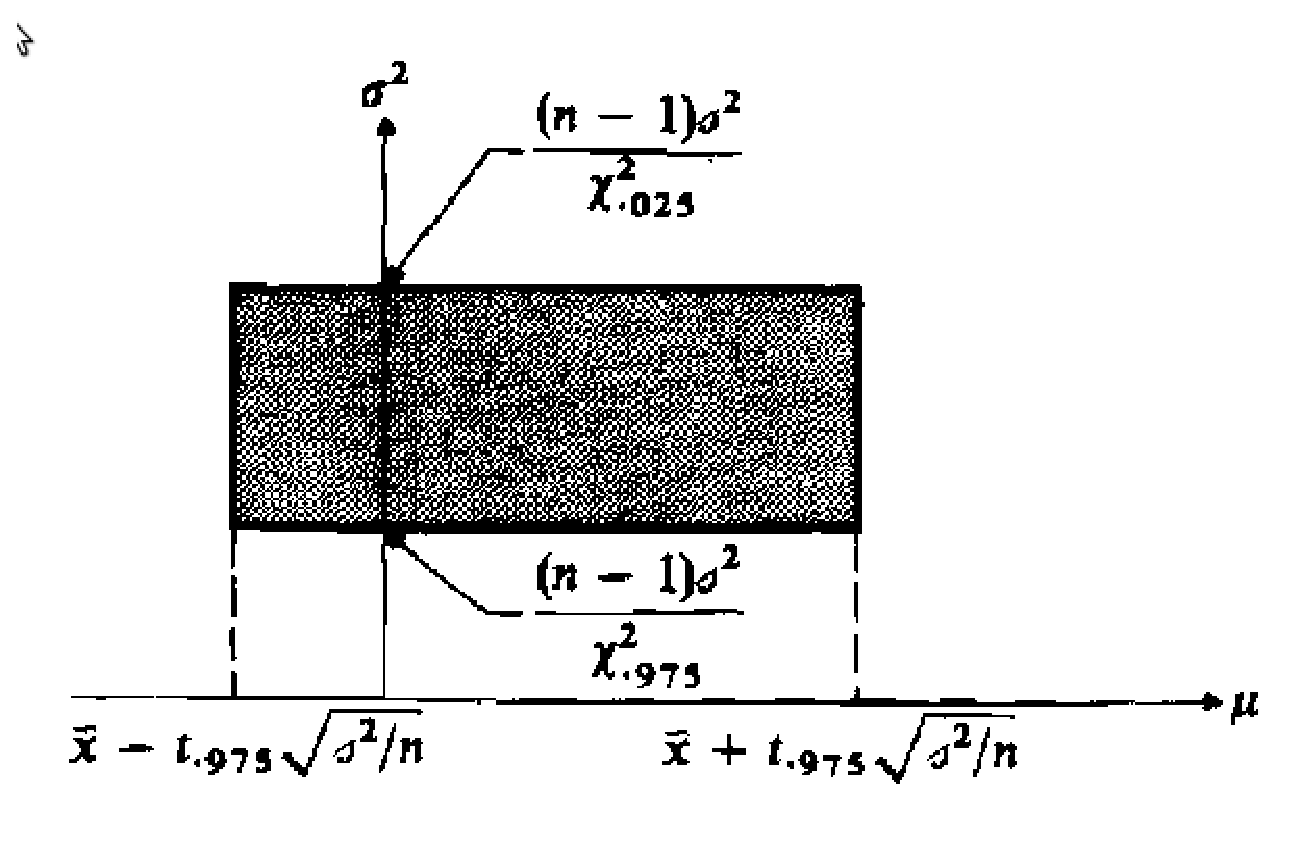
\includegraphics[scale = 0.5]{pictures/conf_interval_mu_sigma_a.eps}
\caption{Region spolehlivosti pro střední hodnotu a rozptyl}
\label{conf-interval-mu-sigma_a}
\end{figure}

Při stanovení regionu spolehlivosti je třeba vzít v potaz vzájemnou nezávislost $\overline{X}$ a $S_n^2$. Protože $Q_1 = \frac{\overline{X} - \mu}{\sigma / \sqrt{n}}$ a $Q_2 = \frac{(n - 1)S_n^2}{\sigma^2}$ představují centrální veličinu, lze nalézt $q_1, q_2'$ a $q_2''$ taková, že
\begin{gather*}
P \left[-q_1 < \frac{\overline{X} - \mu}{\sigma / \sqrt{n}} < q_1 \right] = \gamma_1\\
P \left[q_2' < \frac{(n - 1)S_n^2}{\sigma^2} < q_2'' \right] = \gamma_2
\end{gather*}
Protože jsou $Q_1$ a $Q_2$ vzájemně nezávislé, je jejich sdružená pravděpodobnost rovna
\begin{equation*}
P\left[-q_1 < \frac{\overline{X} - \mu}{\sigma / \sqrt{n}} < q_1, q_2' < \frac{(n - 1)S_n^2}{\sigma^2} < q_2'' \right] = \gamma_1 \gamma_2
\end{equation*}
Čtyři nerovnosti ve výše uvedeném výrazu určují region spolehlivosti, který ilustruje šedivá plocha obrázku (\ref{conf-interval-mu-sigma_b}).

\begin{figure}[htp]
\centering
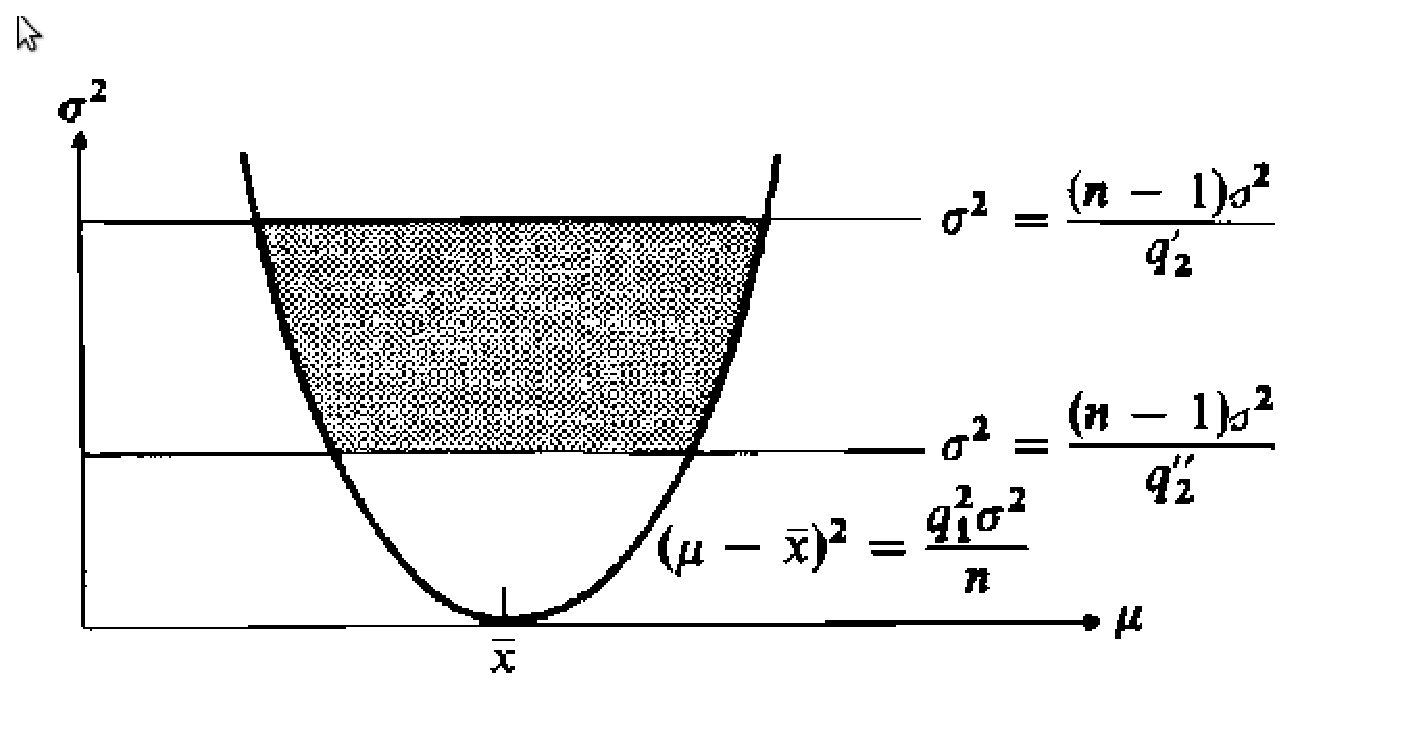
\includegraphics[scale = 0.5]{pictures/conf_interval_mu_sigma_b.eps}
\caption{Region spolehlivosti pro střední hodnotu a rozptyl}
\label{conf-interval-mu-sigma_b}
\end{figure}

Pro $(\mu, \sigma)$ bychom odvodili region spolehlivosti stejně jako v případě $(\mu, \sigma^2)$. Jediným rozdílem by bylo, že bychom pro osu $y$ použili $\sigma$ namísto $\sigma^2$ a parabola z obrázku (\ref{conf-interval-mu-sigma_b}) by se změnila na dvojici polopřímek daných rovnicemi $\mu = \overline{x} \pm q_1 \frac{\sigma}{\sqrt{n}}$, které se protínají v bodě $\overline{x}$ a ose $\mu$.

Závěrem je třeba zdůraznit, že region, který jsme zkonstruovali, nemá pro daná $\gamma_1$ a $\gamma_2$ minimální plochu. Výhoda výše popsaného postupu však spočívá v jeho jednoduchosti a ve skutečnosti, že pro přijatelně veliký náhodný výběr se takto získaný region spolehlivosti příliš neliší od minimálního regionu spolehlivosti. Minimální region spolehlivosti má přibližně eliptický tvar a jeho odvození je poměrně komplikované.

\subsection{Interval spolehlivosti pro rozdíl středních hodnot}

\subsubsection{Dva nezávislé náhodné výběry}

Uvažujme náhodný výběr $X_1, ..., X_m$ z normálního rozdělení se střední hodnotou $\mu_1$ a rozptylem $\sigma^2$ a náhodný výběr $Y_1, ..., Y_n$ z normálního rozdělení se střední hodnotou $\mu_2$ a rozptylem $\sigma^2$. Předpokládejme, že tyto dva náhodné výběry jsou vzájemně nezávislé. Pokusme se nalézt interval spolehlivosti pro $\mu_2 - \mu_1$.

Náhodná veličina $\overline{Y} - \overline{X}$ je normálně rozdělená se střední hodnotou $\mu_2 - \mu_1$ a rozptylem $\frac{\sigma^2}{n} + \frac{\sigma^2}{m}$. Náhodná veličina $\frac{\sum (X_i - \overline{X})^2}{\sigma^2}$ sleduje chi-kvadrát rozdělení s $m - 1$ stupni volnosti a náhodná veličina $\frac{\sum (Y_i - \overline{Y})^2}{\sigma^2}$ sleduje chi-kvadrát rozdělení s $n - 1$ stupni volnosti. Proto náhodná veličina $\frac{\sum (X_i - \overline{X})^2}{\sigma^2} + \frac{\sum (Y_i - \overline{Y})^2}{\sigma^2}$ sleduje chi-kvadrát rozdělení s $m + n - 2$ stupni volnosti. A konečně náhodná veličina
\begin{gather*}
Q = \frac{\frac{(\overline{Y} - \overline{X}) - (\mu_2 - \mu_1)}{\sqrt{\sigma^2/m + \sigma^2/n}}}{\sqrt{\frac{\sum_{i = 1}^n (X_i - \overline{X})^2 + \sum_{i = 1}^n(Y_i - \overline{Y})^2}{\sigma^2(m + n - 2)}}}\\
= \frac{(\overline{Y} - \overline{X}) - (\mu_2 - \mu_1)}{\sqrt{\left(\frac{1}{m} + \frac{1}{n} \right)\frac{\sum_{i = 1}^n(X_i - \overline{X})^2 + \sum_{i = 1}^n (Y_i - \overline{Y})^2}{m + n - 2}}}\\
= \frac{(\overline{Y} - \overline{X}) - (\mu_2 - \mu_1)}{\sqrt{\left(\frac{1}{m} + \frac{1}{n} \right)S_n^{'2}}}
\end{gather*}
sleduje studentovo rozdělení s $m + n - 2$ stupni volnosti. Z toho vyplývá $\gamma = P[-t_{(1 + \gamma) / 2} < Q < t_{(1 + \gamma) / 2}]$, kde $t_{(1 + \gamma) / 2}$ představuje $(1 + \gamma) / 2$ procentní kvantil studentova rozdělení s $m + n - 2$ stupni volnosti. $S_n^{'2}$ je nezkreslená funkce odhadu společného rozptylu $\sigma^2$. Dvojice nerovností
\begin{equation*}
- t_{(1 + \gamma) / 2} < \frac{(\overline{y} - \overline{x}) - (\mu_2 - \mu_1)}{\sqrt{(1/m + 1/n)\mathit{s}^{'2}}} < t_{(1 + \gamma)/2}
\end{equation*}
implikuje
\begin{equation*}
(\overline{y} - \overline{x}) - t_{(1 + \gamma) / 2} \sqrt{\left(\frac{1}{m} + \frac{1}{n} \right)\mathit{s}^{'2}} < \mu_2 - \mu_1 < (\overline{y} - \overline{x}) +  t_{(1 + \gamma) / 2} \sqrt{\left(\frac{1}{m} + \frac{1}{n} \right)\mathit{s}^{'2}}
\end{equation*}
a proto
\begin{equation*}
\left((\overline{Y} - \overline{X}) - t_{(1 + \gamma) / 2} \sqrt{\left(\frac{1}{m} + \frac{1}{n} \right)S_n^{'2}}, (\overline{Y} - \overline{X}) + t_{(1 + \gamma) / 2} \sqrt{\left(\frac{1}{m} + \frac{1}{n}\right)S_n^{'2}}\right)
\end{equation*}
představuje 100$\gamma$ procentní interval spolehlivosti pro $\mu_2 - \mu_1$.

Až dosud jsme předpokládali dva nezávislé náhodné výběry. Nyní předpokládejme, že $(X_1, Y_1), ..., (X_n, Y_n)$ je náhodný výběr z dvourozměrného normálního rozdělení s parametry $\mu_1 = E[X], \mu_2 = E[Y], \sigma_1^2 = D[X], \sigma_2^2 = D[Y]$ a $\rho = \frac{cov[X,Y]}{\sigma_1 \sigma_2}$. Pokusme se nalézt interval spolehlivosti pro $\mu_2 - \mu_1$. Definujme $D_i = Y_i - X_i$ pro $i = 1, ..., n$. Pak $D_1, ..., D_n$ jsou nezávislé náhodné veličiny, které sledují normální rozdělení se střední hodnotou $\mu_D = \mu_2 - \mu_1$ a rozptylem $\sigma_D^2 = \sigma_1^2 + \sigma_2^2 - 2 \rho \sigma_1 \sigma_2$. Na náhodné veličiny $D_1, ..., D_n$ tak lze aplikovat postup z kapitoly (8.2.1). 100$\gamma$ procentní interval spolehlivosti pro $\mu_2 - \mu_1$ je tedy
\begin{equation*}
\left(\overline{D} - t_{(1 + \gamma) / 2} \sqrt{\frac{\sum_{i = 1}^n (D_i - \overline{D})^2}{n(n - 1)}}, \overline{D} + t_{(1 + \gamma) / 2} \sqrt{\frac{\sum_{i = 1}^n (D_i - \overline{D})^2}{n(n - 1)}}\right)
\end{equation*}
kde $t_{(1 + \gamma) / 2}$ představuje $(1 + \gamma) / 2$ procentní kvantil studentova rozdělení s $n - 1$ stupni volnosti.

\section{Metody stanovení intervalu spolehlivosti}

\subsection{Metoda centrální veličiny}

V předchozím textu jsme popsali metodu centrální veličiny pro stanovení intervalu spolehlivosti. Otázkou však zůstává, zda-li vůbec, v kontextu daného problému, centrální veličina existuje.

\begin{corollary}
Uvažujme náhodný výběr $X_1, ..., X_n$ z populace $f(\cdot, \theta)$. Předpokládejme, že kumulativní distribuční funkce $F(x, \theta)$, která odpovídá pravděpodobnostní funkci $f(x, \theta)$, je spojitá v $x$. Pak je zřejmé, že $F(X_i, \theta)$ sleduje uniformní rozdělení nad intervalem $(0, 1)$, a proto $-\ln \left(F(X_i, \theta) \right)$ sleduje pravděpodobnostní rozdělení $e^{-u}I_{(0, \infty)}(u)$, což vyplývá ze vztahu
\begin{equation*}
P[-\ln \left(F(X_i, \theta) \right) \ge u] = P[\ln \left(F(X_i, \theta)\right) \le -u] = P[F(X_i, \theta) \le e^{-u}] = e^{-u}
\end{equation*}
kde $u > 0$. Lze dokázat, že $-\sum \ln \left(F(X_i, \theta)\right)$ sleduje gamma rozdělení s parametry $n$ a 1, tj.
\begin{gather*}
P \left[-\ln(q_2) < - \sum_{i = 1}^n \ln \left(F(X_i, \theta)\right) < -\ln(q_1)\right]\\
= \int_{-\ln(q_2)}^{-\ln(q_1)}\frac{1}{\Gamma(n)}z^{n - 1}e^{-z}dz = P \left[q_1 < \prod_{i = 1}^n F(X_i, \theta) < q_2 \right]
\end{gather*}
pro $0 < q_1 < q_2 < 1$. Proto jsou $\prod_{i = 1}^n F(X_i, \theta)$ a $-\sum_{i = 1}^n \ln \left(F(X_i, \theta)\right)$ centrální veličiny.
\end{corollary}

Z výše uvedeného tvrzení vyplývá, že pokud je kumulativní pravděpodobnostní funkce výběrové populace spojitá, centrální veličina existuje.

\begin{corollary}
Jestliže je kumulativní pravděpodobnostní funkce výběrové populace monotónní v $\theta$ pro libovolné $x$, pak je $\prod_{i = 1}^n F(x_i, \theta)$ taktéž monotónní v $\theta$ pro libovolná $x_1, ..., x_n$. Tato monotónnost umožňuje nalezení intervalu spolehlivosti pro $\theta$. Nerovnosti $q_1 < \prod_{i = 1}^n F(x_i, \theta) < q_2$ totiž, jak ilustruje obrázek (\ref{pivot-quantity-existence}), pak implikují $\mathfrak{t}_1(x_1, ..., x_n) < \theta < \mathfrak{t}_2(x_1, ..., x_n)$. 
\end{corollary}

\begin{figure}[htp]
\centering
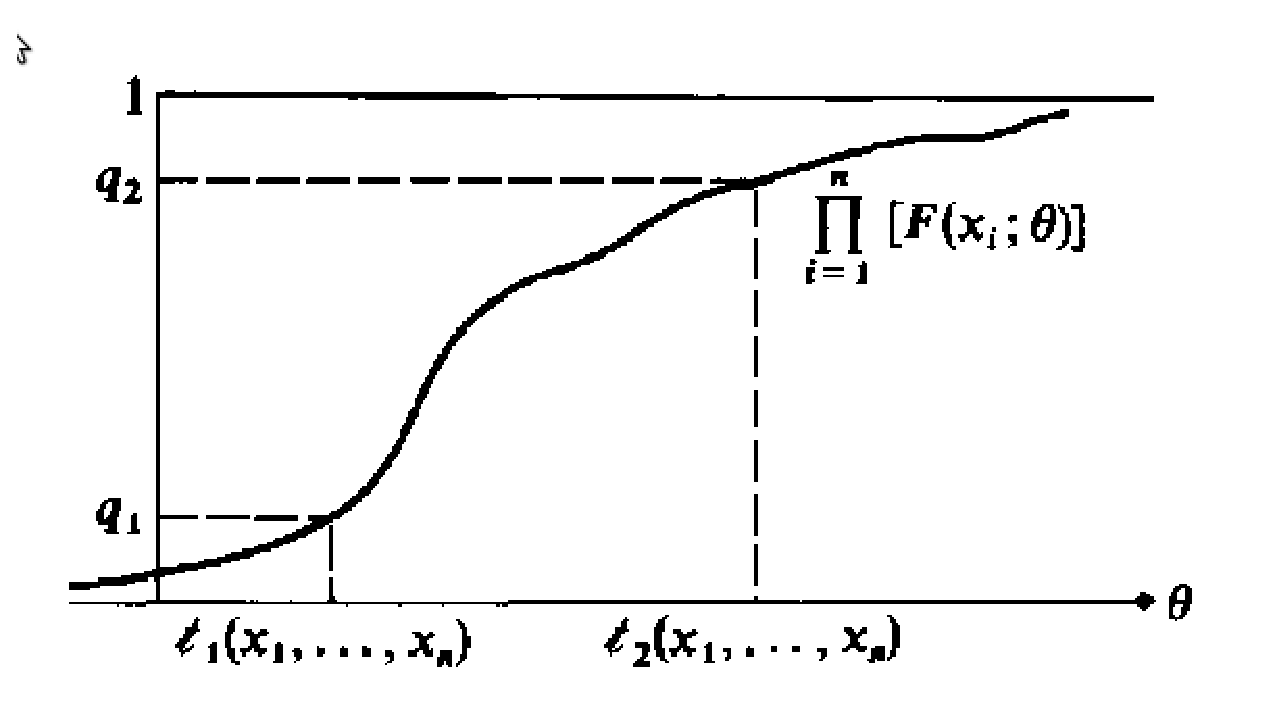
\includegraphics[scale = 0.5]{pictures/pivot_quantity_existence.eps}
\caption{Inverze pravděpodobnostní funkce}
\label{conf-interval-mu-sigma_a}
\end{figure}

\begin{example}
Uvažujme náhodný výběr $X_1, ..., X_n$ z populace $f(x, \theta) = \theta x^{\theta - 1}I_{(0, 1)}(x)$. Odpovídající kumulativní distribuční funkce má tedy tvar $F(x, \theta) = x^{\theta}I_{(0, 1)}(x) + I_{[1, \infty)}(x)$. Jestliže jsou $q_1$ a $q_2$ vybrány tak, že
\begin{gather*}
\gamma = P\left[q_1 < \prod_{i = 1}^n F(X_i, \theta) < q_2 \right] = P\left[q_1 < \prod_{i = 1}^n X_i^{\theta} < q_2 \right]\\
= P \left[\ln(q_1) < \theta \ln \left(\prod_{i = 1}^n X_i \right) < \ln(q_2)\right] = P \left[-\ln(q_2) < -\theta \ln \left(\prod_{i = 1}^n X_i \right) < -\ln(q_1) \right]\\
= P \left[\frac{\ln(q_2)}{\ln \left(\prod_{i = 1}^n X_i \right)} < \theta < \frac{\ln(q_1)}{\ln\left(\prod_{i = 1}^n X_i \right)}\right]
\end{gather*}
pak
\begin{equation*}
 \left(\frac{\ln(q_2)}{\ln \left(\prod_{i = 1}^n X_i\right)}, \frac{\ln(q_1)}{\ln\left(\prod_{i = 1}^n X_i \right)}\right)
\end{equation*}
představuje 100$\gamma$ procentní interval spolehlivosti pro $\theta$.
\end{example}

Závěrem uveďme poznámku ohledně existence centrální veličiny. Jestliže je $\theta$ lokační parametr, pak pravděpodobnostní funkce náhodné veličiny $X_i - \theta$ nezávisí na $\theta$, a proto je centrální veličinou stejně jako např. $\sum X_i - n \theta, Y_j - \theta$ a $Y_1 + Y_n - 2 \theta$. Jestliže je $\theta$ škálovací parametr, pak je pravděpodobnostní funkce náhodné veličiny $X_i / \theta$ nezávislá na $\theta$, a proto se jedná centrální veličinu. Centrálními veličinami jsou v tomto případě také $\sum X_i / \theta, Y_j / \theta$ apod.

\subsection{Statistiká metoda}

Opět uvažujme náhodný výběr $X_1, ..., X_n$ z populace $f(\cdot, \theta_0)$. Předpokládejme, že $\theta_0$, které v následujícím textu představuje skutečnou hodnotu parametru $\theta$, je reálné číslo a že $\overline{\underline{\Theta}}$ představuje interval na reálné ose. Pokusme se stanovit interval spolehlivosti pro $\theta_0$.

Nechť $T = \mathfrak{t}(X_1, ..., X_n)$ představuje statistiku, kterou vybereme jedním z následujících dvou způsobů. Jestliže existuje jednorozměrná dostatečná statistika, pak tuto statistiku použijeme namísto $T$. Jestliže dostatečná statistika neexistuje, pak pro $T$ použijeme bodovou funkci odhadu pro $\theta$. Konkrétní volba statistiky $T$ může také záviset na tom, jak složitá je její aplikace při konstrukci intervalu spolehlivosti - kritickým bodem je zejména odvození její pravděpodobnostní funkce.

Nechť $f_T(t, \theta)$ představuje pravděpodobnostní funkci statistiky $T$\footnote{V následujícím textu budeme předpokládat, že $T$ je spojitá náhodná veličina. Analogický postup však lze aplikovat také v případě nespojité náhodné veličiny.}. Definujme funkce $h_1(\theta)$ a $h_2(\theta)$, pro které platí
\begin{gather*}
\int_{-\infty}^{h_1(\theta)}f_T(t, \theta)dt = p_1\\
\int_{h_2(\theta)}^{\infty}f_T(t, \theta)dt = p_2\\
\end{gather*}
kde $p_1$ a $p_2$ jsou daná reálná čísla, která splňují podmínky $0 < p_1, 0 < p_2$ a $p_1 + p_2 < 1$. $h_1(\theta)$ a $h_2(\theta)$ lze znázornit jako funkce parametru $\theta$. Předpokládejme, že $h_1(\theta)$ a $h_2(\theta)$ jsou rostoucí funkce, pro které navíc platí $h_1(\theta) < h_2(\theta)$. Příklad dvou takovýchto funkcí ilustruje obrázek (\ref{h(1)-h(2)}).
\begin{figure}[htp]
\centering
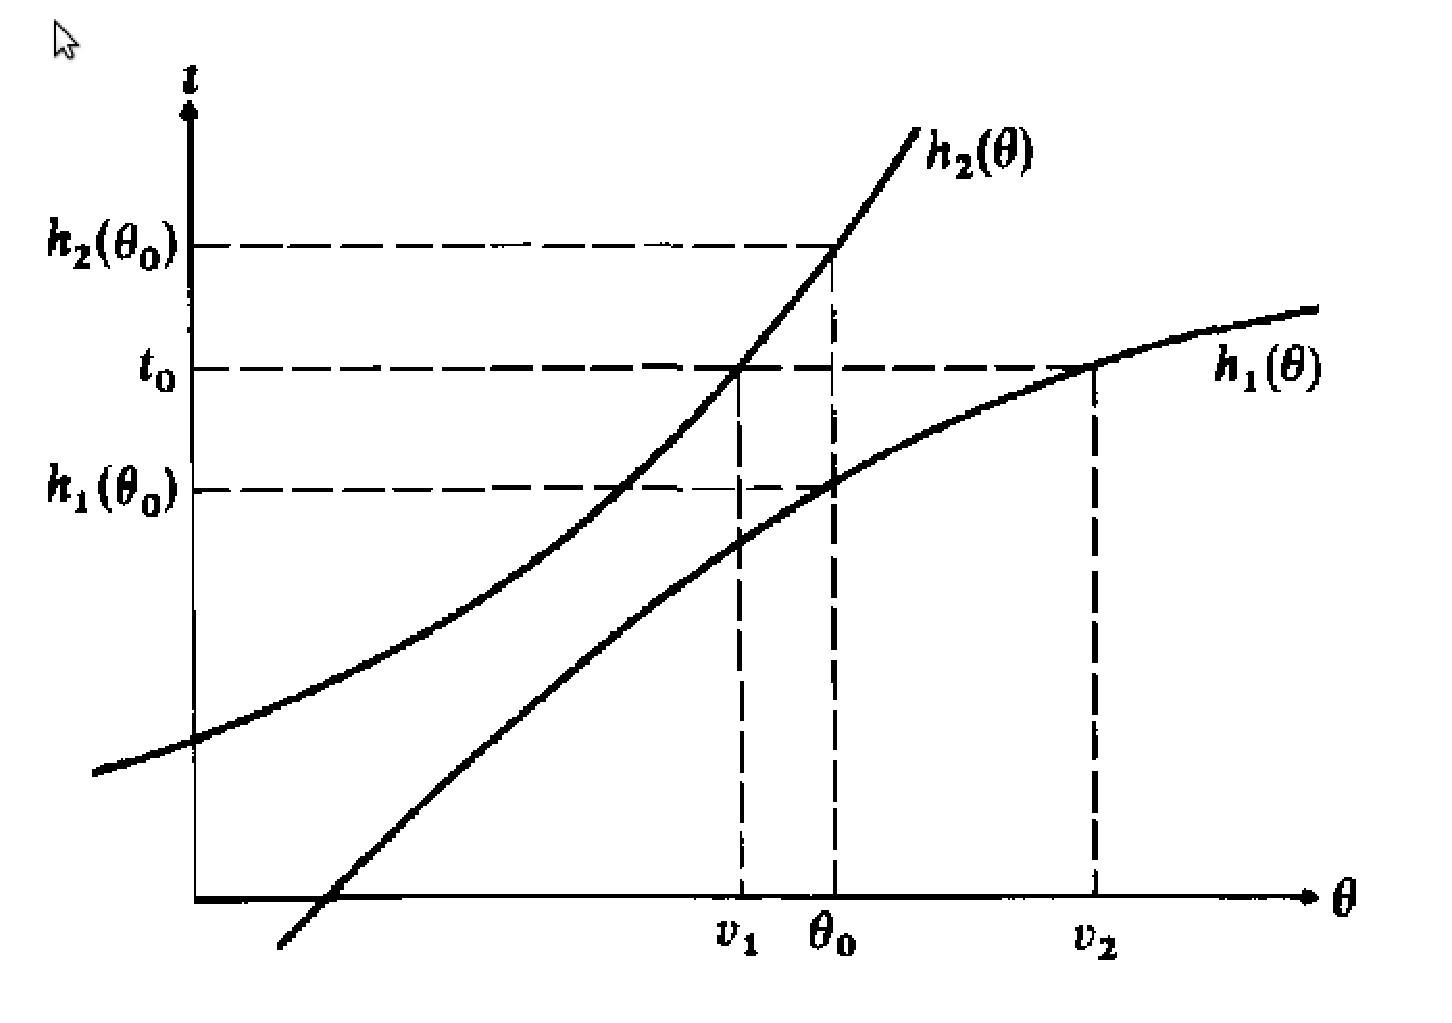
\includegraphics[scale = 0.5]{pictures/h(1)_h(2).eps}
\caption{Graf funkcí $h_1(\cdot)$ a $h_2(\cdot)$}
\label{h(1)-h(2)}
\end{figure}
Nechť $t_0$ označuje hodnotu statistiky $T$, tj. $t_0 = \mathfrak{t}(x_1, ..., x_n)$. Z této hodnoty lze, jak ilustruje obrázek (\ref{h(1)-h(2)}), získat hodnoty $v_1$ a $v_2$ takové, že $v_1 = \mathit{v_1(t_0)}$ a $v_1 = \mathit{v_2(t_0)}$. Z obrázku je dále zřejmé, že $h_1(\theta_0) < t_0 = \mathfrak{t}(x_1, ..., x_n) < h_2(\theta_0)$ platí pouze tehdy a jen tehdy, jestliže $v_1 = \mathit{v_1}(x_1, ..., x_n) < \theta_0 < v_2 = \mathit{v_2}(x_1, ..., x_n)$ pro libovolnou realizaci náhodného výběru $x_1, ..., x_n$. Z definice $h_1(\cdot)$ a $h_2(\cdot)$ však vyplývá
\begin{equation*}
P_{\theta_0}[h_1(\theta_0) < \mathfrak{t}(X_1, ..., X_n) < h_2(\theta_0)] = 1 - p_1 - p_2
\end{equation*}
a proto
\begin{equation*}
P_{\theta_0}[\mathit{v_1}(X_1, ..., X_n) < \theta_0 < \mathit{v_2}(X_1, ..., X_n)] = 1 - p_1 - p_2
\end{equation*}
Interval $(V_1, V_2)$ pak představuje 100$(1 - p_1 - p_2)$ procentní interval spolehlivosti pro $\theta_0$, kde $V_i = \mathit{v_i}(X_1, ..., X_n)$ pro $i = 1, 2$.

\begin{example}
Uvažujme náhodný výběr z populace $f(x, \theta_0) = \frac{1}{\theta_0}I_{(0, \theta_0)}(x)$. Pokusme se stanovit interval spolehlivosti pro $\theta_0$.

O $Y_n = \max(X_1, ..., X_n)$ víme, že se jedná o dostatečnou statistiku a že se jedná o funkci odhadu parametru $\theta_0$ založenou na metodě maximální věrohodnosti. Jestliže použijeme $Y_n$ jakožto statistiku $T$, pak
\begin{equation*}
f_T(t, \theta) = n \left(\frac{t}{\theta}\right)^{n - 1}\frac{1}{\theta}I_{(0, \theta)}(t)
\end{equation*}
$\int_0^{h_1(\theta)}n t^{n - 1}\theta^{-n}dt = p_1$ implikuje $\int_0^{h_1(\theta)}t^{n - 1}dt = \frac{\theta^n p_1}{n}$, což implikuje $\frac{\left(h_1(\theta) \right)^n}{n} = \frac{\theta^n p_1}{n}$ neboli $h_1(\theta) = \theta p_1^{1/n}$. Podobně $p_2 = \int_{h_2(\theta)}^{\theta}nt^{n - 1}\theta^{-n}dt$ implikuje $\theta^n - [h_2(\theta)]^n = \theta^n p_2$ neboli $h_2(\theta) = \theta(1 - p_2)^{1/n}$. Situaci ilustruje obrázek (\ref{h(1)-h(2)-example}), který je konkretizací obrázku (\ref{h(1)-h(2)}) v kontextu našeho příkladu.
\begin{figure}[htp]
\centering
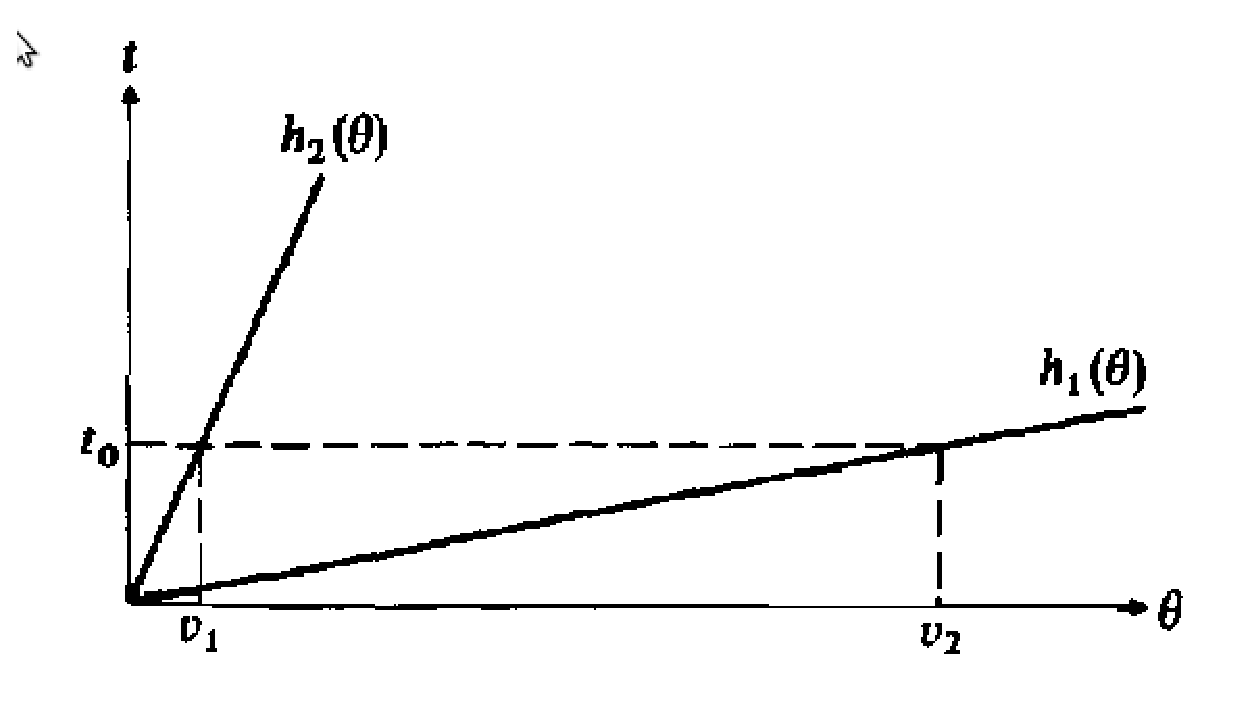
\includegraphics[scale = 0.5]{pictures/h(1)_h(2)_example.eps}
\caption{Graf funkcí $h_1(\cdot)$ a $h_2(\cdot)$}
\label{h(1)-h(2)-example}
\end{figure}
Pro $t_0 = \max(x_1, ..., x_n)$ je $v_1$ definováno jako $h_2(v_1) = t_0$, tj. $h_2(v_1) = v_1(1 - p_2)^{1/n} = t_0$ neboli $v_1 = t_0(1 - p_2)^{-1/n}$. Podobně lze odvodit $v_2 = t_0 p_1^{-1/n}$. To znamená, že 100$(1 - p_1 - p_2)$ procentní interval spolehlivosti pro $\theta_0$ je dán intervalem $(Y_n(1 - p_2)^{-1/n}, Y_n p_1^{-1/n})$.

Naším dalším cílem je stanovit $p_1$ a $p_2$ tak, aby interval spolehlivosti
\begin{equation*}
L = Y_n[p_1^{-1/n} - (1 - p_2)^{-1/n}]
\end{equation*}
byl pokud možno co nejkratší při splnění podmínek $1 - p_1 - p_2 = \gamma$ a $0 < p_1 + p_2 < 1$. To je splněno pro $p_2 = 0$ a $p_1 = 1 - \gamma$.
\end{example}

Z výše uvedeného příkladu je zřejmé, že funkce $h_1(\theta)$ a $h_2(\theta)$ nejsou vlastně potřeba. Pro danou hodnotu $t_0 = \mathfrak{t}(x_, ..., x_n)$ statistiky $T$ je zapotřebí nalézt $v_1 = \mathfrak{v}_1(x_1, ..., x_n)$ a  $v_2 = \mathfrak{v}_2(x_1, ..., x_n)$. $v_2$ lze získat řešením rovnice $p_1 = \int_{-\infty}^{h_1(\theta) = t_0} f_T(t, \theta) dt$ pro $\theta$. Podobně $v_2$ lze získat řešením rovnice $p_2 = \int_{h_(\theta) = t_0}^{\infty}f_T(t, \theta)dt$.

Výše uvedený postup lze aplikovat také pro nespojité náhodné veličiny. Jediným rozdílem bude nahrazení integrálů sumami.

\begin{example}
Uvažujme náhodný výběr $X_1, ..., X_n$ z Bernoulliho rozdělení $P[X = 1] = \theta_0 = 1 - P[X = 0]$. Víme, že $T = \sum X_i$ je dostatečná statistika s binomickým rozdělením, tj.
\begin{equation*}
P[T = t] = \binom{n}{t} \theta_0^t (1 - \theta_0)^{n - t}
\end{equation*}
pro $t = 0, 1, ..., n$. Pokusme se stanovit interval spolehlivosti pro $\theta_0$.

Předpokládejme, že $T = t_0$. Řešme rovnice
\begin{gather*}
p_1 = \sum_{t = 0}^{t_0} \binom{n}{t}\theta^t(1 - \theta)^{n - 1}\\
p_2 = \sum_{t = 0}^{t_0} \binom{n}{t}\theta^t(1 - \theta)^{n - 1}\\
\end{gather*}
pro $\theta$. Jestliže např. $p_1 = 0.0509, p_2 = 0.0159, n = 20$ a $T = 4$, pak je 93.33 procentní interval spolehlivosti parametru $\theta_0$ dán intervalem $(0.05, 0.40)$.
\end{example}

\section{Interval spolehlivosti pro výběry velkého rozsahu}

V případě bodového odhadu jsme ukázali, že v některých případech je možné nalézt posloupnost funkcí odhadu $T_n = \mathfrak{t}_n(X_1, ..., X_n)$ pro parametr $\theta$ pravděpodobnostního rozdělení $f(\cdot, \theta)$, které sledují asymptoticky normální rozdělení. To znamená, že $T_n$ asymptoticky sleduje normální rozdělení se střední hodnotou $\theta$ a rozptylem $\sigma_n^2(\theta)$. V kapitole (7.8) jsme ukázali, že v případě náhodného výběru velkého rozsahu sleduje funkce odhadu $\hat{\Theta}_n = \hat{\zeta}_n (X_1, ..., X_n)$ založená na metodě maximální věrohodnosti přibližně normální rozdělení se střední hodnotou $\theta$ a rozptylem
\begin{equation*}
\sigma_n^2(\theta) = \frac{1}{n E_{\theta}\left[\left(\frac{\partial}{\partial \theta}\ln\left(f(X, \theta)\right) \right)^2 \right]}
\end{equation*}
V tomto případě lze $\frac{T_n - \theta}{\sigma_n(\theta)}$ použít jako přibližnou centrální veličinu a příslušný 100$\gamma$ procentní interval spolehlivosti získat z nerovností
\begin{equation*}
-z < \frac{T_n - \theta}{\sigma_n(\theta)} < z
\end{equation*}
kde $z = z_{(1 + \gamma)/2}$ je definováno jako $\Phi(z_{(1 + z) / 2}) = (1 + \gamma) / 2$ neboli $\Phi(z) - \Phi(-z) = \gamma$. Tento postup lze aplikovat vždy, když lze z výše uvedených nerovností izolovat $\theta$.

\begin{example}
Uvažujme náhodný výběr $X_1, ..., X_n$ z populace $f(x, \theta) = \theta e^{-\theta x}I_{(0, \infty)}(x)$. Z příkladu (7.55) víme, že funkce odhadu dle metody maximální věrohodnosti pro $\theta$ má tvar $1 / \overline{X}_n$ a asymptoticky sleduje normální rozdělení se střední hodnotou $\theta$ a rozptylem
\begin{equation*}
\sigma_n^2(\theta) = \frac{1}{n E_{\theta}\left[\left(\frac{\partial}{\partial \theta} \ln \left(f(X, \theta)\right)\right)^2\right]} = \frac{\theta^2}{n}
\end{equation*}
Proto
\begin{gather*}
\gamma \approx P\left[-z < \frac{1 / \overline{X}_n - \theta}{\sqrt{\theta^2/n}} < z \right]\\
= P\left[-\frac{z \theta}{\sqrt{n}} < \frac{1}{\overline{X}_n} - \theta < \frac{z \theta}{\sqrt{n}} \right]\\
= P\left[\frac{1 / \overline{X}_n}{1 + z/\sqrt{n}} < \theta < \frac{1 / \overline{X}_n}{1 - z / \sqrt{n}} \right]
\end{gather*}
V případě náhodného výběru velkého rozsahu tak má 100$\gamma$ procentní interval spolehlivosti pro parametr $\theta$ tvar
\begin{equation*}
\left(\frac{1 / \overline{X}}{1 + z/\sqrt{n}}, \frac{1 / \overline{X}}{1 - z / \sqrt{n}}\right)
\end{equation*}
kde $z$ je definováno jako $\Phi(z) - \Phi(-z) = \gamma$.
\end{example}

\begin{example}
Uvažujme náhodný výběr velkého rozsahu z Bernoulliho rozdělení s parametry $\theta = P[X = 1] = 1 - P[X = 0]$. Funkce odhadu pro $\theta$ dle metody maximální věrohodnosti má tvar $\hat{\Theta} = \overline{X}_n$ a její rozptyl je $\sigma_n^2(\theta) = \theta(1 - \theta)/n$. 100$\gamma$ procentní interval spolehlivosti pro $\theta$ lze získat z nerovností
\begin{equation*}
P \left[\frac{2n \hat{\Theta} + z^2 - z \sqrt{4n \hat{\theta} + z^2 - 4n \hat{\Theta}^2}}{2(n + z^2)} < \theta < \frac{2n \hat{\Theta} + z^2 + z \sqrt{4n \hat{\theta} + z^2 - 4n \hat{\Theta}^2}}{2(n + z^2)} \right] \approx \gamma
\end{equation*}
Vzhledem k tomu, že předmětem našeho zájmu je náhodný výběr velkého rozsahu, lze všechny členy výše uvedených nerovností, které obsahují $1/\sqrt{n}$ resp. $1 / n$, zanedbat. Tím se dostáváme k
\begin{equation*}
P\left[\hat{\Theta} - z \sqrt{\frac{\hat{\Theta} - (1 - \hat{\Theta})}{n}} < \theta < \hat{\Theta} + z \sqrt{\frac{\hat{\Theta}(1 - \hat{\Theta})}{n}} \right] \approx \gamma
\end{equation*} 
\end{example}
Vztah odvozený ve výše uvedeném příkladě je vztahem, který bychom získali, pokud bychom v $\sigma_n^2(\theta)$ použily $\hat{\Theta}$ namísto $\theta$. Tato substituce by implikovala, že $\frac{\hat{\Theta} - \theta}{\sqrt{\hat{\Theta}(1 - \hat{\Theta})/n}}$ je přibližně normálně rozdělené s nulovou střední hodnotou a jednotkovým rozptylem. Tento závěr, který však nebudeme dokazovat, je obecně platný. To znamená, že funkce odhadu $\hat{\Theta}$ dle metody maximální věrohodnosti asymptoticky sleduje normální rozdělení se střední hodnotou $\theta$ a rozptylem $\sigma_n^2(\theta)$, který lze v případě náhodného výběru dostatečně velkého rozsahu aproximovat pomocí $\sigma_2^n(\Theta)$. Je zřejmé, že toto zjištění velmi zjednoduší konstrukci intervalu spolehlivosti, protože
\begin{equation*}
P\left[-z < \frac{\hat{\Theta} - \theta}{\sigma_n(\hat{\Theta})} < z \right] \approx \gamma
\end{equation*}
lze snadno převést do tvaru
\begin{equation*}
P[\hat{\Theta} - z \sigma_n(\hat{\Theta}) < \theta < \hat{\Theta} + z \sigma_n(\hat{\Theta})] \approx \gamma
\end{equation*}

Závěrem uveďme, že interval spolehlivosti pro náhodný výběr velkého rozsahu založený na funkci odhadu dle metody maximální věrohodnosti je optimální. To znamená, že je v průměru kratší než interval spolehlivosti založený na alternativních funkcích odhadu.

\section{Bayesovský interval}

Následující text navazuje na kapitolu (7.6). Uvažujme náhodný výběr z pravděpodobnostní funkce $f(\cdot|\theta)$, jejíž funkční předpis je znám. Připomeňme, že $\theta$ je hodnota náhodné veličiny $\Theta$, která je charakterizována apriorní pravděpodobnostní funkcí $g_{\Theta}(\cdot)$. Posteriorní pravděpodobnostní funkce náhodné veličiny $\Theta$ pro dané $(X_1, ..., X_n) = (x_1, ..., x_n)$ má tvar
\begin{equation*}
f_{\Theta|X_1 = x_1, ..., X_n = x_n}(\theta|x_1, ..., x_n) = \frac{\left[\prod_{i = 1}^n f(x_i|\theta) \right]}{\int \left[\prod_{i = 1}^n f(x_i|\theta) \right]g_{\Theta}(\theta)d\theta}
\end{equation*}
Pro fixní $\gamma$ je libovolný interval $(t_1, t_2)$ splňující podmínku
\begin{equation*}
\int_{t_1}^{t_2}f_{\Theta|X_1 = x_1, ..., X_n = x_n}(\theta|x_1, ..., x_n)d\theta = \gamma
\end{equation*}
100$\gamma$ procentním Bayesovským intervalem odhadu pro prameter $\theta$. V praxi bychom se snažili zvolit taková $t_1$ a $t_2$, aby délka intervalu byla co nejmenší. Dále platí, že $t_i = \mathit{t_i}(x_1, ..., x_n)$, tj. na $t_i$ lze pohlížet jako na funkci pozorování $x_1, ..., x_n$.

\begin{example}
Uvažujme náhodný výběr $X_1, ..., X_n$ z normálního rozdělení se střední hodnoto $\theta$ a jednotkovým rozptylem. Předpokládejme, že $\Theta$ má normální rozdělení se střední hodnotou $x_0$ a rozptylem 1. Pokusme se odhadnout $\theta$.

Z příkladu (7.48) víme, že posteriorní rozdělení náhodné veličiny $\Theta$ sleduje normální rozdělení se střední hodnotou $\frac{\sum_{i = 0}^n}{n + 1}$ a rozptylem $\frac{1}{n + 1}$. Hledáme $t_1$ a $t_2$, která splňují podmínku
\begin{gather*}
\gamma = \int_{t_1}^{t_2} f_{\Theta|X_1 = x_1, ..., X_n = x_n}(\theta|x_1, ..., x_n)d\theta\\
= \Phi\left(\frac{t_2 - \sum_{i = 0}^n \frac{x_i}{n + 1}}{\sqrt{1 / (n + 1)}}\right) - \Phi\left(\frac{t_1 - \sum_{i = 0}^n \frac{x_i}{n + 1}}{\sqrt{1 / (n + 1)}}\right)
\end{gather*}
Jestliže zvolíme $z$ takové, že $\Phi(z) - \Phi(-z) = \gamma$, pak
\begin{gather*}
t_2 = \frac{\sum_{i = 0}^n x_i}{n + 1} + z\sqrt{\frac{1}{n + 1}}\\
t_1 = \frac{\sum_{i = 0}^n x_i}{n + 1} - z\sqrt{\frac{1}{n + 1}}
\end{gather*}
definuje nejkratší Bayesovský interval odhadu pro $\theta$. Odpovídající interval spolehlivosti založený na metodě maximální věrohodnosti je dán intervalem $\left(\frac{\sum x_i}{n} - z\sqrt{\frac{1}{n}}, \frac{\sum x_i}{n} + z\sqrt{\frac{1}{n}} \right)$. Jediný rozdíl mezi těmito dvěma metodami spočívá v tom, že v případě Baysovského intervalu je velikost náhodného výběru zdánlivě navýšena o jedna, kde toto ``dodatečné'' pozorování je představováno střední hodnotou apriorního normálního rozdělení náhodné veličiny $\Theta$. 
\end{example}
